\begin{figure}[htbp]
\section*{ FZD5}
\centering
\begin{subfigure}[b]{0.95\textwidth}
\centering
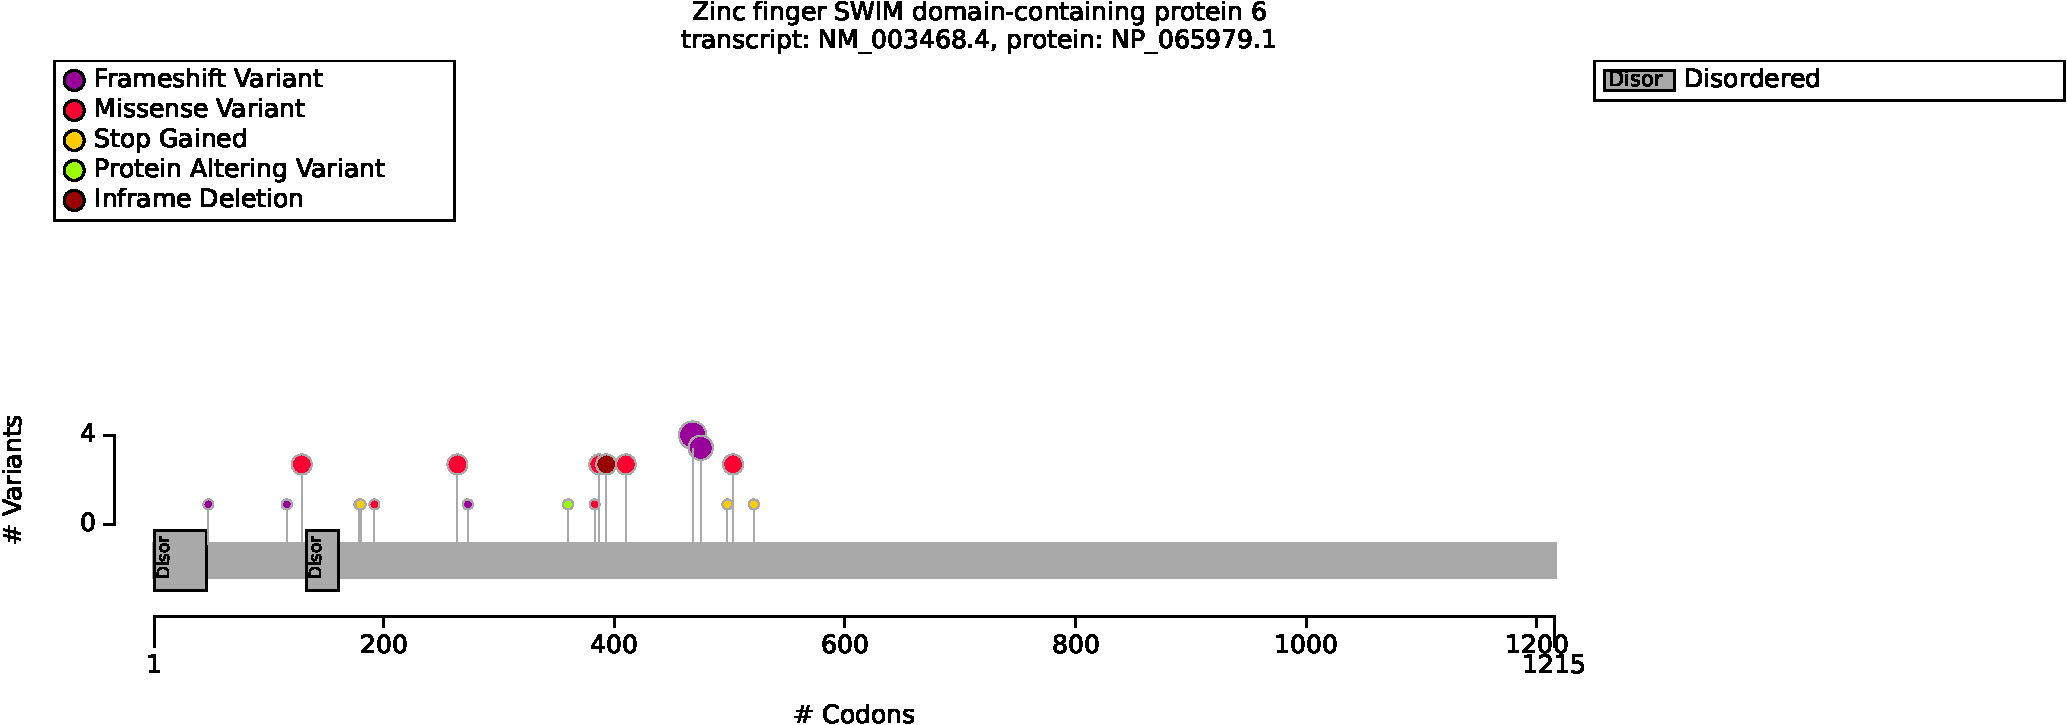
\includegraphics[width=\textwidth]{ img/FZD5_protein_diagram.pdf} 
\captionsetup{justification=raggedright,singlelinecheck=false}
\caption{Distribution of variants in FZD5}
\end{subfigure}

\vspace{2em}

\begin{subfigure}[b]{0.95\textwidth}
\centering
\resizebox{\textwidth}{!}{
\begin{tabular}{llllrr}
\toprule
Genotype (A) & Genotype (B) & total tests performed & significant results\\
\midrule
missense & other & 18 & 0\\
\bottomrule
\end{tabular}
}
\captionsetup{justification=raggedright,singlelinecheck=false}
\caption{Fisher Exact Test performed to compare HPO annotation frequency with respect to genotypes. }
\end{subfigure}

\vspace{2em}

\caption{ The cohort comprised 29 individuals (11 females, 10 males, 8 with unknown sex). A total of 16 HPO terms were used to annotate the cohort. Disease diagnosis: Microphthalmia/coloboma 11 (OMIM:620731). No significant correlations identified. A total of 19 unique variant alleles were found in \textit{FZD5} (transcript: \texttt{NM\_003468.4}, protein id: \texttt{NP\_065979.1}).}
\end{figure}
